% Focused reading copy; substantive sources are shared with the monograph.
\documentclass[12pt,a4paper]{article}
\usepackage[margin=25mm,headheight=15pt]{geometry}
\usepackage{fontspec}
\setmainfont{TeX Gyre Pagella}
\setsansfont{TeX Gyre Heros}
\setmonofont[Scale=0.84]{DejaVu Sans Mono}
\usepackage{amsmath,amssymb,mathtools,microtype,setspace}
\setstretch{1.06}
\usepackage{booktabs,longtable,tabularx,array}
\renewcommand{\arraystretch}{1.2}
\usepackage{graphicx,xcolor,tikz,float}
\usetikzlibrary{arrows.meta,positioning,calc,shapes.geometric}
\usepackage{enumitem,listings,titlesec}
\usepackage[round,authoryear]{natbib}
\usepackage[hyphens]{url}
\Urlmuskip=0mu plus 2mu
\definecolor{navy}{HTML}{173A53}
\definecolor{teal}{HTML}{186C75}
\definecolor{pale}{HTML}{F1F5F6}
\usepackage[unicode,colorlinks=true,linkcolor=navy,citecolor=navy,urlcolor=navy]{hyperref}
\hypersetup{pdftitle={From policy documents to ODRL: review and implementation proposal},pdfauthor={Chak Wong},pdfsubject={2023 SFC-HKMA suitability circular; ODRL, Catala and source-linked policy translation}}
\titleformat{\section}{\Large\sffamily\bfseries\color{navy}\raggedright}{\thesection}{0.7em}{}
\titleformat{\subsection}{\large\sffamily\bfseries\raggedright}{\thesubsection}{0.65em}{}
\setlength{\parindent}{0pt}
\setlength{\parskip}{0.45em}
\setlength{\emergencystretch}{3em}
\setlist{itemsep=0.15em,topsep=0.35em,leftmargin=1.6em}
\newcolumntype{Y}{>{\raggedright\arraybackslash}X}
\newcolumntype{P}[1]{>{\raggedright\arraybackslash}p{#1}}
\lstset{basicstyle=\small\ttfamily,backgroundcolor=\color{pale},frame=single,rulecolor=\color{pale},breaklines=true,columns=fullflexible,keepspaces=true,showstringspaces=false,aboveskip=0.8em,belowskip=0.8em}
\title{\sffamily\bfseries\color{navy}From policy documents to ODRL\\[0.5em]\Large Literature, software and a concrete implementation proposal}
\author{Chak Wong}
\date{22 October 2026}
\begin{document}
\raggedbottom
\maketitle
\begin{abstract}
The 2023 SFC--HKMA suitability circular requires more than extraction of
permissions and prohibitions: its streamlined procedures depend on eligibility,
prior consent, conditional relief and continuing duties. This review examines
text-to-ODRL methods, regulatory profiles, formal semantics and available
software, then proposes a bounded extension to LegalMath using its existing
prospectus evidence machinery and SPI calculations. ODRL is the first proposed
output of a reviewed source-linked interpretation; Catala supplies selected
computations and additional checks. The proposal specifies the profile,
modules, result contracts, worked export, implementation sequence and
counterexamples needed to evaluate the feature. It distinguishes implemented
repository components from proposed ODRL work and structural conformance
from legal fidelity.
\end{abstract}
\clearpage
\tableofcontents
\clearpage
\section{From policy documents to ODRL: what must survive translation}
\label{sec:odrl-review}

The next proposed output of LegalMath is a machine-readable policy in the
Open Digital Rights Language, ODRL. The immediate case is the joint
SFC--HKMA circular of 28 July 2023, reference 23EC35, on the Streamlined
Approach for sophisticated professional investors (SPIs). The useful question
is whether an intermediary may apply particular streamlined procedures to a
client and transaction, and which duties remain. It is not simply whether a
trade is allowed. This difference determines what the translation must express
\citep{sfcspi,sfcspiannex1,sfcspiannex2}.

Consider a designated account whose gross exposure has risen above the client's
streamlining threshold. A sentence-level translator might read the threshold
rule and produce a prohibition on every further transaction. Annex~2 FAQ~6
expressly permits the account to continue operating and executing transactions
while top-ups and deposits are restricted. It does not expect the intermediary
to reduce or unwind exposure for this purpose. An ordinary suitability route
also remains relevant. The missing distinction is the kind of action and the
monitoring arrangement, not a different spelling of the threshold
\citep[FAQ~6]{sfcspiannex2}.

This review therefore recommends \emph{ODRL as the first new deliverable},
produced from a reviewed interpretation linked to the source. Selected Catala
calculations should accompany it. Requiring a complete Catala program first
would postpone the desired policy representation without resolving its
normative questions. Treating ODRL as the only representation of the circular
would instead risk losing meanings that the selected ODRL profile cannot
execute. The implementation proposal below develops a shared interpretation
with explicit projections into these different languages.

\subsection{Scope and strength of the evidence}

The review was completed on 22 October 2026. It combines the circular body,
both annexes, direct text-to-ODRL research, work on regulatory profiles and
formal semantics, and static inspection of selected software. The official
annex PDFs match the repository's archived copies byte for byte. This fixes a
historical translation case; a current operational application would still
need the relevant source editions, amendments and incorporated provisions.
The Code of Conduct, Professional Investor Rules and referenced FAQs must
remain named dependencies rather than silently assumed complete
\citep{hkmaodrlsurvey2026}.

Searches used Crossref, OpenAlex, GitHub, the W3C ODRL community's implementation
landscape, and references from the inspected papers. The recorded
``HKMA ODRL'' query returned no results, and no direct HKMA translation study
was found in the inspected material. This is a targeted survey, not proof
that no such work exists. Eight newly retained papers received technical
reading of the relevant method, semantics and evaluation; existing Catala
and eFLINT papers supplied focused comparisons. Nine public code checkouts
were pinned. Unavailable originals and documentation-only findings remain
identified in the accompanying reading record. No generation experiment or
third-party software benchmark was run \citep{hkmaodrlsurvey2026}.

The important evaluation question is whether a translation preserves the
decision and duty distinctions in the circular. A graph can be valid RDF,
conform to a set of shapes, and still prohibit the transactions that FAQ~6
allows. Conversely, a disagreement between evaluators can reflect different
declared semantics rather than a malformed graph. The following discussion
keeps these questions separate so that published scores are not asked to
answer a question their experiments did not test.

\subsection{ODRL's basic model and the need for a profile}

ODRL is a W3C model for expressing permissions, prohibitions and duties
concerning identifiable resources. An action says what may, may not, or must
be done; a party identifies a participant; an asset identifies the resource
to which the action applies. Constraints restrict when a rule applies.
The same policy can be serialized as JSON-LD, a JSON representation that
maps names to identifiers in an RDF graph. RDF supplies the linked statements;
it does not infer the legal meaning of ``sophisticated investor''
\citep[secs.~2--3]{odrlmodel2018}.

The distinction between two ODRL relationships is particularly important.
A duty attached to a permission through \texttt{odrl:duty} is a prerequisite
for that permission. A duty connected directly to a policy through
\texttt{odrl:obligation} is an independent obligation. Prior written consent
and a later annual review should therefore not be represented as an
undifferentiated list of actions that must all have happened before the first
transaction. The circular and the chosen event interpretation must determine
which performance is needed, by whom and at what time
\citep[secs.~2.6.1, 2.6.4--2.6.5]{odrlmodel2018}.

A \emph{profile} defines additional vocabulary and semantics for a particular
application. The proposed HKMA profile would name applying the Streamlined
Approach, reviewing continued qualification, providing a requested explanation,
and the observations used to establish their conditions. ODRL requires a
processor to understand a declared profile and stop when it does not recognise
it. A new identifier in a JSON file is consequently not enough: the evaluator
needs an implementation of that term's meaning. A profile extends the core;
it is not permission to reverse the meaning of an existing ODRL relationship
\citep[sec.~3]{odrlmodel2018}.

For this case, the resource can be the identified service or procedure instance
to which streamlined treatment applies. The intermediary is the party exercising
that permission; the client and account remain separately identified. Regulatory
source authority should be recorded explicitly in provenance. It should not
be inferred merely by putting the regulator into an \texttt{assigner} field,
which would hide a substantive mapping choice. A general regulatory rule set
can use \texttt{odrl:Set}; a particular agreement with a client is a different
record. These are proposed domain choices to specify and test, rather than
universal mappings supplied by ODRL.

\subsection{The circular contains calculations, dispensations and legal changes}

The financial limb illustrates the calculational part. Let $P$ be the
qualifying portfolio value and $N$ the qualifying net assets excluding the
primary residence, both expressed in Hong Kong dollars at the declared
assessment date. After the ownership, aggregation and currency questions have
been resolved, the financial condition is
\begin{equation}
\label{eq:odrl-financial-limb}
 F(P,N)=(P\geq 40{,}000{,}000)\ \lor\ (N\geq 80{,}000{,}000).
\end{equation}
Equality satisfies either threshold. A portfolio of HK\$40 million therefore
passes this limb even when the net-asset alternative does not. The disjunction
does not establish SPI status: professional-investor status, knowledge or
experience and investment objectives are additional conditions. Joint holdings,
written allocations, liabilities and qualifying investment-holding corporations
require their own source-based treatment
\citep[paras.~1--5]{sfcspiannex1}.

Knowledge or experience can be established through the specified degree or
postgraduate diploma, a professional qualification in finance, at least one
year of relevant professional work in the financial sector, or at least five
transactions within the past three years in the same product category.
Reliance on trading experience therefore needs category identity and a calendar
reference date. A representative's expertise is not automatically the client's
expertise, although transactions through a representative or joint account may
contribute to the client's trading history. Unknown objectives cannot establish
that the client is nonconservative
\citep[paras.~4.1, 5.1 and 7.3]{sfcspiannex1}
\citep[FAQ~2]{sfcspiannex2}.

The procedure relaxations introduce a different kind of statement. Paragraphs
10 and 11 say that specified procedures are ``not required'' under the
applicable conditions. This is a dispensation from a requirement; it is not
a prohibition on performing that procedure. Nor is it a blanket exemption
from suitability obligations. The explanation relaxation has exceptions for
requests and material queries, and solicited or recommended transactions differ
from unsolicited complex-product transactions. A translation must preserve the
scope of the relieved duty and the duties that survive
\citep[paras.~10--11]{sfcspiannex1}.

Client choices also change what applies. Prior written agreement and the
specified explanation precede use of the approach. Paragraph~13.1(d) provides
for withdrawal; paragraphs~13.2(c)(iii) and 13.2(d)(iii) concern changes to
categories and thresholds; paragraph~14 requires annual review and reminders.
An old consent event cannot authorize indefinitely after withdrawal. Equally,
``annually'' does not choose a 365-day arithmetic convention. The selected
calendar and effective-time interpretation must be visible
\citep[paras.~13--14]{sfcspiannex1}.

Finally, the financial evidence requirement must not be strengthened
accidentally. FAQ~1 permits reliance on disclosed information after reasonable
know-your-client efforts in the stated circumstances; inconsistencies need
clarification. Recordkeeping and universally demanding documentary proof are
different requirements. These qualitative assessments need evidence and a
declared interpretation. Inventing a numeric cutoff for ``reasonably satisfied''
would make a program easier to run by changing its subject
\citep[FAQ~1]{sfcspiannex2}.

\subsection{What direct text-to-ODRL research demonstrates}

\citet{revelodrl2023} offer an inspectable translation route: a sentence is
parsed into Abstract Meaning Representation (AMR), converted into RDF, and
transduced into ODRL. AMR makes linguistic relationships explicit before
the policy representation is selected. This is a useful baseline for separating
linguistic analysis from policy construction. It does not remove the need to
resolve definitions, references and the legal effect of exceptions.

Their experiment contains approximately 100 simple deontic sentences, about
20\% handcrafted and the remainder generated from a grammar, plus ten
negative examples. Modality extraction has reported precision 0.780, recall
0.640 and F-score 0.703; action extraction has precision 0.989, recall 0.810
and F-score 0.891. These are component scores rather than whole-policy legal
accuracy. Document preprocessing and definition resolution are described as
hypothetical extensions. The error discussion includes the scope of negation:
permission not to reproduce is different from lack of permission to reproduce.
That problem is directly relevant to the circular's ``not required'' language
\citep[method, experiments and error discussion]{revelodrl2023}.

\citet{mustafaodrl2024} take an ontology-guided language-model approach. They
provide ODRL concepts, curated explanations and examples, then refine generated
policies. Twelve cultural-dataspace use cases, three models and three methods
give 108 configurations; the paper describes initially running each use case
once. Its prominent 91.95\% figure is 217 of 236 selected checks for one use
case with refinement. It is not the probability that a complete legal policy
was interpreted correctly. The method supports a small generation baseline,
especially because it makes the allowed vocabulary explicit
\citep[secs.~2--4 and Table~1]{mustafaodrl2024}.

The associated LLM4ODRL code parses policies and checks SHACL shapes. SHACL
expresses conditions on an RDF graph: for example, whether a particular kind
of node has the required properties. Some repository shapes require creator,
description, title and issue date. Those can be useful application requirements,
but should not all be attributed to the W3C core standard. No repository-level
licence was found in the inspected checkout, so the method can inform a baseline
without assuming permission to copy its code \citep{hkmaodrlsoftware2026}.

\citet{agentodrl2026} add an orchestrator, reference rewriting, decomposition,
ontology-guided generation and SHACL-guided correction. Seventy seed cases are
expanded with a model into 770 cases: 440 simple, 220 with parallel relationships
and 110 with sequential dependencies. The semantic evaluation uses checkpoints
extracted by a model and judgments from two language models; the grammar score
uses selected shape violations. These measurements are useful for the authors'
generation experiment. They are not an independently established legal
interpretation of a circular and its annexes.

AgentODRL also gives a reason to keep the first experiment simple. Fixed
preprocessing workflows achieve higher aggregate semantic scores than the
adaptive orchestrator in parts of the reported comparison. The evidence does
not justify assuming that more orchestration improves this task. Compare a
direct ontology-guided proposal with explicit reference handling before adopting
the full system. Its Apache-licensed code is reusable, but the inspected
correction loop can retain a final candidate after exhausting its correction
budget without establishing success. The local result must preserve that failure
status. Reference rewriting must also retain the passages that supplied each
condition and exception \citep{agentodrl2026,hkmaodrlsoftware2026}.

There is earlier NLP work on RDF licence generation by Cabrio, Aprosio and
Villata, discussed in the AMR paper. Its original technical text was not
obtained in this survey, so it is a historical lead rather than separately
verified performance evidence. Likewise, De Vos, Kirrane, Padget and Satoh's
2019 \emph{ODRL Policy Modelling and Compliance Checking} is a directly
relevant lead on regulatory profiles and answer-set-program compliance,
including GDPR. The publication record and later references were located,
but the original attachment remained unavailable. Detailed claims about its
encoding or adoption would require that text
\citep{revelodrl2023,hkmaodrlsurvey2026}.

\subsection{Legal meaning and formal semantics constrain the translation}

\citet{criticalodrl2021} explain why a legal relationship can exceed a simple
usage permission. Duties, institutional powers, delegation, revocation and
policy lifecycle require distinctions that are easily hidden by a single
allow/deny result. For this circular, withdrawing consent changes the
arrangement; a dispensation changes which procedure is required; and the
regulator, intermediary and client occupy different roles. The critique
identifies modelling questions. Later semantics work must be considered
alongside it rather than assuming ODRL has remained unchanged.

The inspected AIUP profile supplies a practical example of regulatory
specialisation. It defines vocabulary for intended and precluded AI uses,
oversight and reporting, while expressly limiting its coverage of the EU AI
Act. Its draft specification, rather than the associated research paper, was
the source inspected here. Its relevance is the discipline of declaring exact
domain terms and supported questions. A corresponding HKMA profile should
state which duties and changes it can represent, rather than call every
operation \texttt{odrl:use} \citep{aiupprofile2024}.

\citet{bonattiodrl2025} develop declarative semantics for rule activation,
action matching, duties and compliance over traces. A trace records relevant
events and their order. This makes an otherwise hidden question explicit:
does one performance of a duty permit one subsequent action or many? A consent
to a continuing arrangement and an explanation in response to a particular
request require different answers. Their discussion also distinguishes
constraints on activation from conditions of fulfilment, considers policy gaps,
and identifies unresolved features such as temporal operands and a separate
meaning for \texttt{andSequence}. These are proposed semantic choices, not
a new W3C Recommendation
\citep[sec.~3, especially 3.6--3.8]{bonattiodrl2025}.

\citet{odrlnormalisation2026} show how a restricted policy fragment can be
normalised and compared under declared semantics. Their algorithms partition
numerical and symbolic conditions into matching regions and establish
preservation results. This suggests future checks for overlapping threshold
conditions or an unintended change between exports. The fragment excludes
attached duties, remedies and consequences; standalone obligations remain
unchanged in the policy-preservation result. Splitting one obligation into
several required obligations can change its meaning. The normal form can grow
exponentially in the number of attributes, and empirical performance evaluation
is left for future work. This is a basis for restricted comparison, not a
generic equivalence procedure for the whole circular
\citep[secs.~3--4, especially Theorem~6]{odrlnormalisation2026}.

LegalRuleML and eFLINT help identify what the internal interpretation should
retain even when the initial export is narrower. LegalRuleML addresses source
correspondence, context, defeasibility, authority and alternative readings.
The original eFLINT work separates action compliance from duty compliance
and represents events that create or terminate normative relationships.
Thus a transaction decision and an outstanding review duty can be reported
separately. These ideas support the internal design; this proposal does not
make a new LegalRuleML serializer or eFLINT runtime a prerequisite
\citep{legalruleml2021,eflint2020}.

\subsection{Evaluation software: what to reuse and what to test first}

\citet{oval2026} formalise access decisions and offline and streaming monitoring,
and present the OVAL implementation. Its algorithm processes events while
tracking rule matches and outstanding requirements. That is closer to the
circular's combination of procedure eligibility and continuing duties than
syntax validation alone. The reported evaluation uses synthetic workloads and
comparison with the SolidLab/FORCE cases. Agreement is 54 of 68 cases after
mapping the comparison system's ``not enough information'' to false. Different
reasoning and duty interpretations account for disagreements. Runtime results
on these workloads therefore cannot establish greater legal correctness
\citep[secs.~4--6]{oval2026}.

The pinned October OVAL code is a reasonable first candidate for a bounded
trial. Its access API defaults to accepting unfulfilled duties on a promise of
future fulfilment; another setting requires prior performance. The default
must not decide whether written consent can be obtained after the transaction.
Missing values can become false or remain null depending on configuration;
\texttt{andSequence} is implemented as conjunction rather than temporal
sequence; event counting is not a category-specific rolling three-year
history. Numeric comparisons attempt floating-point conversion, even where
older feature documentation describes lexical comparison. Explicit units,
some temporal operands and other constructs are unsupported. The proposal
therefore supplies exact calculations and a declared event adapter, with
unsupported terms reported before evaluation \citep{hkmaodrlsoftware2026}.

FORCE offers a useful testing pattern: a policy, request, state of the world
and expected compliance report. Its current documentation describes limitations
on duties, while code includes duty-reporting structures and rules. Reporting
a duty and enforcing it as a prerequisite to permission are distinct
capabilities. A helper also connects policy-level duties through
\texttt{odrl:duty}, where the W3C model uses \texttt{odrl:obligation}.
These are concrete compatibility checks for the intended input route, not
evidence that every FORCE evaluation fails. The reported 67/68
activation-similarity result is not a local result or a measure of fulfilled
legal duties. The associated 2025 papers were located bibliographically but
not obtained in full, so the recommendation rests on inspected code and
documentation \citep{hkmaodrlsoftware2026}.

ODRE addresses the connection between descriptive policy terms and executable
values. \citet{odre2024} use runtime interpolation and operand/action adapters,
with Python and Java implementations and 24 demonstration tests per
implementation. Their tested enforcement is synchronous; temporal monitoring
is future work in that version. The Python checkout presents additional static
concerns: the rule traversal discards whether a rule was reached through
permission, prohibition or obligation, and the constraint query appears to
look directly on a rule where its own sample uses a nested constraint node.
An empty constraint result is then accepted. These findings were not executed
as failures, but they are sufficient to withhold selection as the first general
normative evaluator pending focused reproduction
\citep{odre2024,hkmaodrlsoftware2026}.

Eclipse Dataspace Components provides registered evaluation functions,
execution scopes and JSON-LD policy transformation. These are useful later
if the product needs dataspace negotiation or transfer services. They do not
extract a circular's norms or define SPI qualification. pySHACL is the smaller
immediate dependency for graph validation; its shapes must be reviewed and
must actually target the intended policy nodes. The public ODRL-shape
repository is a source of ideas, but no repository-level licence was found
in the inspected checkout \citep{hkmaodrlsoftware2026}.

\begin{table}[htbp]
\centering
\caption{Selection for a first trial, based on static inspection rather than a benchmark ranking.}
\label{tab:odrl-software-choices}
\begingroup
\footnotesize
\renewcommand{\arraystretch}{1.08}
\begin{tabularx}{\textwidth}{P{27mm}YY}
\toprule
Component & Proposed use & Condition before reliance\\
\midrule
\href{https://github.com/keman-ruc/wanle-Agentodrl}{AgentODRL} & Generation and reference-handling ideas & Preserve source maps and failed correction status.\\
\href{https://github.com/Daham-Mustaf/LLM4ODRL}{LLM4ODRL} & Simple ontology-guided methodological baseline & Resolve licence before copying code; review shape assumptions.\\
\href{https://github.com/RDFLib/pySHACL}{pySHACL} & Structural and profile checks & Review shapes, targeting and negative cases.\\
\href{https://github.com/DIPS-Tools/ODRL-Engine}{OVAL} & First evaluator trial & Pin duty/default semantics; supply exact facts and explicit time handling.\\
\href{https://github.com/odrl-force/ODRL-Evaluator}{FORCE} & Scenario/report design and second evaluator & Establish duty and policy-obligation behavior on the chosen route.\\
\href{https://github.com/ODRE-Framework/odre-python}{ODRE} & Operand-adapter design reference & Reproduce and resolve the inspected traversal concerns.\\
\href{https://github.com/eclipse-edc/Connector}{EDC} & Later deployment integration & Supply the domain semantics; justify the larger integration cost.\\
\bottomrule
\end{tabularx}
\endgroup
\end{table}

The inspected AgentODRL, pySHACL documentation, ODRE and EDC declare Apache-2.0
licensing; OVAL and FORCE use MIT. The table links to the public repositories.
The proposed first OVAL trial is pinned to \texttt{b2838782b7ce}; the maintained
AgentODRL checkout is \texttt{d55ed231ba7d}, FORCE is \texttt{194894a04588},
and ODRE Python is \texttt{1a2cb06004f0}. All nine full checkout commits and inspected-file
hashes are retained in the survey manifest. These snapshots fix what was
examined, not a promise about a later release. No software is ranked as
production ready on this evidence \citep{hkmaodrlsoftware2026}.

\subsection{Choosing the relationship with Catala}

Catala is valuable where the circular gives computations with defaults and
exceptions. Equation~\ref{eq:odrl-financial-limb}, explicit allocation rules
and category histories are candidates once their premises are fixed. The
Catala paper's compilation result concerns translation between formal calculi.
It does not prove that a natural-language source was interpreted correctly
or that another language has the same semantics
\citep[secs.~4.2--4.5]{catala2021}.

Translating the document into Catala first gives early executable calculations
and uses existing tooling. It is attractive for a predominantly computational
source or an already reviewed Catala model. Here, however, a calculation need
not retain the distinction between a dispensation, a legal power to withdraw,
and an outstanding duty. Reconstructing that information later for ODRL can
lose meaning. Catala-first is therefore an unnecessary prerequisite for this
circular.

ODRL-first followed by Catala delivers the desired interchange representation
early and makes parties, actions and duties visible. But any meaning omitted
from ODRL is also missing from the subsequent calculation. Agreement between
the two generated outputs mainly tests that translation step. Fully separate
document-to-ODRL and document-to-Catala processes provide more independence,
but duplicate interpretation work and permit sources, terminology and
assumptions to drift. They are useful experimental comparators on a small
fragment, rather than the preferred everyday authoring process.

The recommended design retains a richer reviewed interpretation and exports
ODRL while invoking Catala for selected calculations. Independent scenario
specifications challenge both. This separates four questions: whether the
graph conforms to its profile, whether the evaluator implements the chosen
semantics, whether the two computations agree on a declared domain, and
whether the interpretation is supported by the circular. Catala can help
answer the third and expose defects relevant to the second. It does not
establish the first or fourth by itself.

The practical consequence is to begin with source coverage and the FAQ~6,
consent and explanation counterexamples. The initial feature should produce a
reviewable policy and an explicit account of what it cannot express. A generic
ODRL-to-Catala compiler is not required to obtain that result.
Section~\ref{sec:odrl-proposal} specifies the records, modules and checks
needed to make this recommendation concrete.

\section{Proposed feature: source-linked ODRL for the SPI circular}
\label{sec:odrl-proposal}

The proposed feature accepts a versioned policy-document bundle and produces
a draft ODRL policy together with the source interpretation, supported scope
and evaluation evidence needed to inspect it. The first bundle is circular
23EC35 and its two annexes. The first question is whether the Streamlined
Approach is available under stated premises and what particular duties remain.
The feature should not label its answer as general permission to trade.
It should retain unresolved interpretations and observations as part of the
answer rather than replace them with plausible defaults.

The review above supplies the basis for this design. Ontology-guided drafting
is an established research approach, but its reported structural and
model-judged scores do not establish source fidelity. ODRL evaluators also make
different choices about duties and missing information. The proposed extension
therefore adds deterministic policy export and explicit evaluator adapters
around an interpretation that remains richer than the executable fragment.
All ODRL modules, commands and examples in this section are proposed work.
The source, translation and SPI components identified as existing were
inspected in the repository; no ODRL runtime was executed for this proposal
\citep{hkmaodrlsurvey2026,hkmaodrlsoftware2026}.

\subsection{Start from the work that already exists}

The inspected main commit is \texttt{3c3e462acabf}; the prospectus branch
\path{feature/prospectus-evidence-master} is at \texttt{e8beb52b1339}.
That prospectus commit is an ancestor of the inspected main commit, and the
committed \path{src/legalmath/prospectus} and
\path{src/legalmath/translation} trees have no differences between them.
The relevant code is already available on main. This comparison does not
assert that unrelated worktree changes or every branch file are identical
\citep{hkmaodrlsoftware2026}.

The prospectus successor modules already preserve source identity and
occurrences. \path{source_graph.py} retains document hashes, page and line
locations, geometry and time information; \path{construction_ast.py},
\path{reference_closure.py} and \path{priorities.py} preserve source assembly,
dependencies and proposed overrides. These mechanisms can keep an annex
qualification attached to the paragraph it explains. They need new circular,
FAQ and incorporated-source roles. A later date or a generic priority edge
must not decide legal priority without an interpretation.

The clause graph provides a useful starting record for actors, affected
parties, modality, conditions, exceptions and source spans. Its recogniser is
currently a bounded bond grammar with effects such as principal loss,
conversion and repayment. It is not already a general regulatory parser.
The extension should reuse its source-occurrence checks while introducing
regulatory norm types separately. This avoids turning a bond-specific
\texttt{effect} field into an unexplained catch-all.

There is more direct reuse in \path{prospectus/models.py} and
\path{prospectus/semantics.py}. The financial model uses inclusive alternatives
and integer Hong Kong dollar cents. The client model combines professional
investor status, financial qualification, knowledge or experience and
objectives. The threshold model already distinguishes a designated account
without new funds from the ordinary exposure comparison. Selected duty
models distinguish suitability matching, due diligence and explanation relief.
These models explicitly identify themselves as conditional synthetic
specifications. Their source bindings leave legal entailment and completeness
unestablished; ownership, currency conversion, valid monitoring arrangements
and other applicable requirements remain premises
\citep{hkmaodrlsoftware2026}.

Their exact threshold expression is particularly useful for a first regression
case. Let $G$ be gross exposure and $M$ the streamlining threshold in integer
HKD cents. Let $D$ mean that the designated-account arrangement and its
required controls are valid, and $A$ mean that the request adds funds. Under
those declared premises the existing amount-condition model is
\begin{equation}
\label{eq:odrl-existing-threshold}
 T(G,M,D,A)=(G\leq M)\ \lor\ (D\land\neg A).
\end{equation}
If $G$ is HK\$12 million and $M$ HK\$10 million, the first term is false.
A transaction within a valid designated account without new funds can still
satisfy the second term. A top-up does not. This is an illustrative conditional
calculation: gross exposure must include leverage and the required treatment
of transferred-out noncash investments, and $D$ must not be set true merely
because an account has a convenient name. The source for the exception must
include FAQ~6, alongside the threshold and monitoring provisions
\citep[paras.~8.1--8.5]{sfcspiannex1}
\citep[FAQs~6--7]{sfcspiannex2}.

The shared \emph{LegalRuleModel} already retains typed facts, expressions,
scope, source spans and interpretations. Its capabilities include exact
amounts and declared date/collection operations on supported targets.
\path{translation/pipeline.py} currently accepts only RuleIR and Catala;
its build path assumes those executable targets. An ODRL export must therefore
be a separate adapter with its own result type, not a new string added to
the target list while retaining assumptions about Java builds.
\path{translation/verification.py} accepts external expected outcomes and
checks execution and replay; \path{prospectus/checks.py} contains independently
written symbolic expressions and deliberate mutations. These are useful
patterns, not an existing ODRL conformance suite
\citep{hkmaodrlsoftware2026}.

The lifecycle, duty-performance and amendment modules provide additional
patterns for preserving events, evidence and changed decisions. They require
explicit bindings to this circular. Prospectus analysis also contributes
substantive evidence: Annex~2 FAQ~3 calls for distinct product categories for
debt instruments with loss-absorption features. Evidence of contractual
write-down or conversion can inform that classification. A paragraph match
alone is insufficient; the operative product terms and reviewed category
rule must support the assigned category \citep[FAQ~3]{sfcspiannex2}.

\subsection{Keep norms and calculations connected but distinct}

The proposed internal addition is a \emph{PolicyInterpretation}, containing
versioned norm records and links to existing calculation models. Each norm
has a stable identity, exact source occurrences, the wording and interpreted
modality, actor and affected parties, action and object, applicability,
conditions, exceptions, timing and evidence requirements. It also records
unresolved questions and the source of any priority. A duty records its
trigger, required performance and how evidence establishes that performance.
A client power records which state it changes, such as consent withdrawal.
A dispensation names the particular duty it qualifies.

These records should reference typed calculations by model and rule identity.
The financial norm can refer to the existing inclusive threshold calculation,
while the interpretation retains the legal conditions for counting each
holding. A generated Boolean called \texttt{eligible} is not enough: the
record must preserve the premises that made it true and the source of each
premise. Conversely, copying the complete computational expression into every
ODRL constraint would obscure which part is a calculation and which is a
normative consequence.

Every source unit must receive a disposition: represented in the supported
export, retained as a definition or dependency, deliberately deferred with a
reason, or unresolved. This makes the coverage denominator the source bundle,
not the number of rules the generator happened to produce. The source graph
must retain references to material outside the bundle. Missing dependencies
can leave a conditional policy useful for research while preventing a claim
to have represented every applicable requirement.

The following architecture keeps these responsibilities visible. The
independent cases enter after the interpretation has been fixed; they must
not be generated merely by reading back the same expression being tested.

\begin{figure}[htbp]
\centering
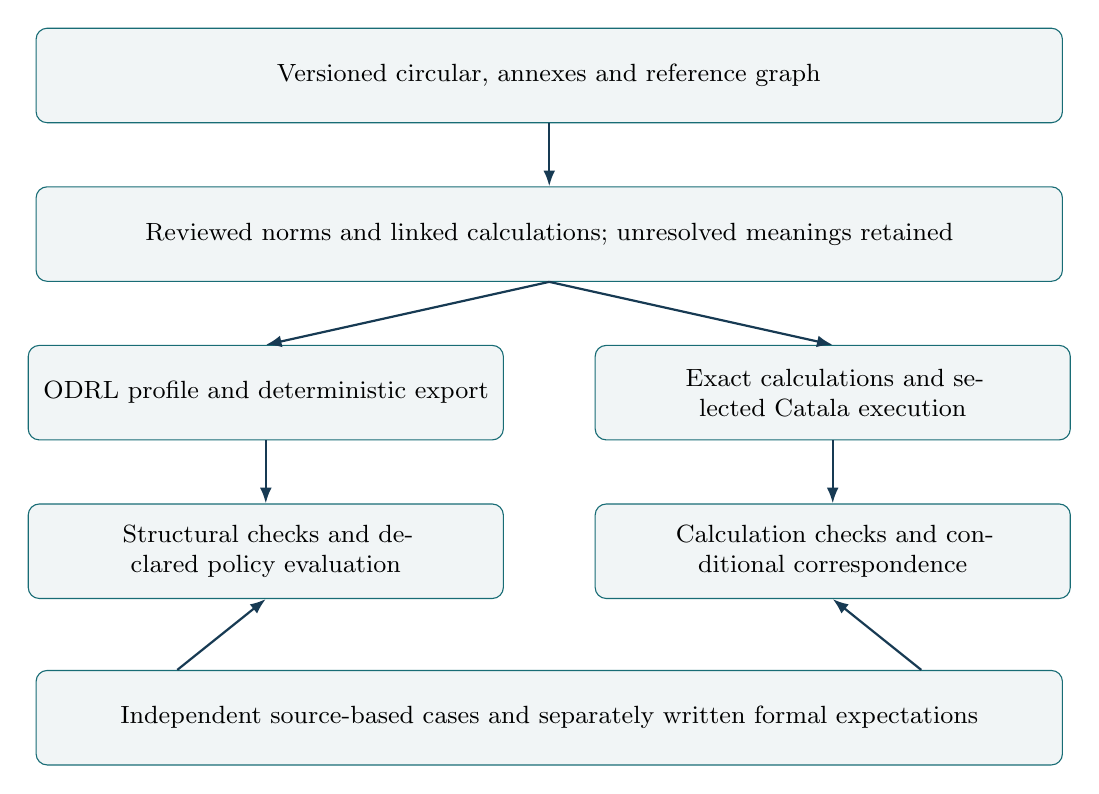
\begin{tikzpicture}[node distance=8mm and 12mm,
 box/.style={draw=teal,fill=pale,rounded corners,align=center,
 text width=58mm,minimum height=12mm,font=\small},
 wide/.style={box,text width=128mm},
 arr/.style={-{Latex[length=2mm]},thick,draw=navy}]
\node[wide] (sources) {Versioned circular, annexes and reference graph};
\node[wide,below=of sources] (meaning) {Reviewed norms and linked calculations; unresolved meanings retained};
\node[box,below=8mm of meaning.south,xshift=-36mm] (odrl) {ODRL profile and deterministic export};
\node[box,below=8mm of meaning.south,xshift=36mm] (catala) {Exact calculations and selected Catala execution};
\node[box,below=of odrl] (evaluate) {Structural checks and declared policy evaluation};
\node[box,below=of catala] (checks) {Calculation checks and conditional correspondence};
\node[wide,below=9mm of $(evaluate.south)!0.5!(checks.south)$] (cases) {Independent source-based cases and separately written formal expectations};
\draw[arr] (sources)--(meaning);
\draw[arr] (meaning.south)--(odrl.north);
\draw[arr] (meaning.south)--(catala.north);
\draw[arr] (odrl)--(evaluate);
\draw[arr] (catala)--(checks);
\draw[arr] (cases.north west)++(18mm,0)--(evaluate.south);
\draw[arr] (cases.north east)++(-18mm,0)--(checks.south);
\end{tikzpicture}
\caption{One source interpretation supplies complementary representations.
Independent cases can expose a shared error; agreement between the outputs
alone cannot.}
\label{fig:odrl-proposed-architecture}
\end{figure}

\subsection{Define two supported profiles before generating policies}

The first implementation should distinguish an \emph{eligibility profile}
from a later \emph{duty-monitoring profile}. These are proposed LegalMath
profiles for the historical HKMA case, not profiles issued or endorsed by
HKMA. Their versioned identifiers must bind vocabulary, shapes and executable
semantics together. An evaluator must refuse an unknown profile or an
unsupported construct before returning a legal-facing result.

The eligibility profile supports a permission to apply streamlined procedures
to an identified request. It uses explicit intermediary, client, account,
product-category and decision-time identities. Its conditions consume typed
results for qualification, selected category, threshold treatment, continuing
consent and other declared prerequisites. Monetary and calendar calculations
are evaluated exactly outside the generic ODRL engine, with provenance and
missing-fact status retained. This is an intentional computational boundary,
not a claim that the engine itself understands joint ownership or currency
conversion.

For the initial profile, use simple named constraints and explicitly defined
conjunctions. Do not emit unsupported arithmetic, \texttt{inheritFrom},
\texttt{rightOperandReference}, temporal \texttt{andSequence}, remedies or
consequences and hope that a consumer ignores them safely. An unknown term
produces an unsupported result. A prohibition is exported only where a
reviewed interpretation establishes the prohibited action and its scope;
failure to establish streamlined eligibility does not create a trading
prohibition.

The duty-monitoring profile extends this with named triggers and correlated
performance events. Prior consent is verified as an effective prerequisite;
annual review is a separately triggered obligation. An explanation duty is
linked to the relevant request or material query and its required response.
Evidence of a different explanation for a different transaction cannot
satisfy it. Recurrence, deadlines and continued validity need explicit rules
in the domain event adapter. A duty is fulfilled only when its required
performance is established, rather than when the duty becomes active.

Dispensations require special care. The first implementation should calculate
the applicable set of ordinary procedures and their conditional relief in
the internal norm model, then export the supported remaining duties. It must
retain a mapping from each relieved duty to the source and condition granting
relief. If the ordinary duty's source has not been resolved, the result stays
conditional. A custom \emph{dispensation} extension can be considered later
if interchange requires it, but only with defined semantics and evaluator
support. It must never be approximated by a prohibition on the relieved action.

For general policies use \texttt{odrl:Set}, with regulatory authority in
source provenance and party roles explicitly mapped by the profile. For a
concrete export, the assignee is the intermediary and the target is the
identified streamlined-service request. Client and account identities remain
bound in that request and its evidence record. The permission allows applying
the procedure, so the target cannot silently change into the investment itself.
These choices make the scope of the result inspectable.

\subsection{A worked export makes the interface concrete}

Suppose that a synthetic client and transaction satisfy the reviewed
non-amount premises: professional-investor status, knowledge or experience,
objectives, selected category and continuing prior agreement. The request
is an internal transaction in a valid designated account, adding no funds,
with the HK\$12 million gross exposure and HK\$10 million threshold described
above. Equation~\ref{eq:odrl-existing-threshold} supplies the amount condition.
The example also assumes the declared other requirements have been established;
they are not automatically set true by the exporter.

The following JSON-LD illustrates the proposed eligibility-profile output.
The \texttt{example.org} identifiers are reserved illustrative names. The
inline context maps every abbreviated name to its RDF identifier, so the
example does not rely on downloading an unspecified context. It is a design
fragment, not a completed or conformance-tested translation of the circular.

\begin{lstlisting}[float=htbp,caption={An illustrative permission to apply a procedure to one request.},label={lst:odrl-permission-fragment}]
{
  "@context": {
    "odrl": "http://www.w3.org/ns/odrl/2/",
    "lm": "https://example.org/legalmath/",
    "prov": "http://www.w3.org/ns/prov#"
  },
  "@id": "lm:policy/spi-example-001",
  "@type": "odrl:Set",
  "odrl:profile": {
    "@id": "lm:profile/hkma-spi-eligibility-v1"
  },
  "prov:wasDerivedFrom": {
    "@id": "lm:interpretation/spi-001"
  },
  "odrl:permission": [{
    "@id": "lm:rule/apply-streamlined-001",
    "odrl:assignee": {"@id": "lm:party/intermediary-001"},
    "odrl:target": {"@id": "lm:request/transaction-001"},
    "odrl:action": {"@id": "lm:applyStreamlinedApproach"},
    "odrl:constraint": [{
      "odrl:leftOperand": {"@id": "lm:streamlinedEligible"},
      "odrl:operator": {"@id": "odrl:eq"},
      "odrl:rightOperand": true
    }]
  }]
}
\end{lstlisting}

The custom left operand is deliberately explicit. Its value is a query against
the linked calculation and evidence record for this exact request, actor,
client, account and decision time. The implementation must retain the
component results and source locations behind it. A model-generated assertion
that \texttt{streamlinedEligible=true} is not an acceptable substitute for
that computation. The export manifest binds the policy bytes, profile version,
norm model, calculation model and provenance map. A consumer without the
profile implementation has a descriptive graph, not an executable permission.

On the declared facts the permission can apply. Changing only the request to
a top-up makes the above-threshold designated-account alternative false.
Changing only the evidence so that consent is missing makes the conclusion
unresolved. Changing only the observation to a documented withdrawal makes
continuing consent false after its effective time. None of these results,
by itself, says that every ordinary-route trade is prohibited.

The result record should expose those distinctions through separate fields.
The proposed permission result has one of \texttt{PERMITTED},
\texttt{NOT\_ESTABLISHED}, \texttt{UNKNOWN}, \texttt{CONFLICT} or
\texttt{UNSUPPORTED}, with rule and premise explanations. An explicit
\texttt{PROHIBITED} result requires an applicable prohibition, not just the
absence of a permission. \texttt{NOT\_ESTABLISHED} here means that the declared
streamlined route fails on known facts. It is not a claim about the ordinary
route. Duty results are reported separately as inactive, pending, fulfilled,
violated or unresolved under the declared event semantics. These result names
are a proposed application contract, not new W3C vocabulary.

\subsection{Consent, missing information and time need executable rules}

The observation boundary should reuse the repository's distinction between
known, unknown and conflicting evidence. The profile evaluates only supported
observations whose subject, effective interval and knowledge time match the
request. A known absence and an unobserved fact are different inputs. A
complete history with four qualifying trades differs from an incomplete
history that happens to contain four. A missing portfolio need not block the
financial limb if the alternative net-assets branch is established, subject
to the declared conflict policy. The existing complete and partial model
profiles must not be mixed implicitly.

Consent requires an event model rather than an everlasting Boolean. Each
record identifies the client, intermediary, agreed categories and threshold,
source evidence, time of execution and effective interval. Withdrawal ends the
relevant consent state according to the declared interpretation. Category or
threshold changes produce new effective states while preserving earlier
decisions. Replaying a Monday transaction should use what applied and was
known on Monday; a later correction can produce a separate reassessment.
The source supplies the rights and procedures, while exact timestamp and
calendar conventions remain explicit implementation choices
\citep[paras.~13.1--14.2]{sfcspiannex1}.

Annual review should create a due obligation according to a documented
calendar rule and the relevant arrangement date. Its performance record must
include the required qualification/agreement checks and written reminders.
The first release should require an explicit assessment of the due date
where the source does not determine a unique calendar convention. Later
calendar automation can replace that input after the convention is specified
and checked. It must not make every future review a prerequisite to the first
transaction or treat the first review as discharging every later one.

This is also why the OVAL trial must explicitly configure duty and
unmatched-request behavior. Where a permission has an attached prerequisite,
the adapter should request evidence of prior fulfilment and test that a future
promise fails. The initial consent implementation can instead use a verified
current-state condition, avoiding an assumption that one generic duty match
models continuing consent. Either mapping needs the same withdrawal cases.
The adapter must document which parts are evaluated by OVAL and which by the
domain state processor; it must not describe the combined result as native
support for a feature the engine lacks \citep{hkmaodrlsoftware2026}.

\subsection{Concrete modules and output contract}

Implement the extension under a new \path{src/legalmath/odrl/} package.
Keep the initial export API separate from the existing Java/Catala build
function, reusing its model validation, source identities and hashing where
appropriate. The following module boundaries are proposed to make the first
change reviewable without refactoring unrelated execution code.

\begin{longtable}{P{31mm}P{117mm}}
\caption{Proposed modules and their first responsibilities.}
\label{tab:odrl-proposed-modules}\\
\toprule
Module & Responsibility and principal output\\
\midrule
\endfirsthead
\toprule
Module & Responsibility and principal output\\
\midrule
\endhead
\bottomrule
\endfoot
\path{model.py} & Versioned PolicyInterpretation and Norm records; source/exception links; typed references to existing calculation rules; coverage and unresolved questions.\\
\path{profile.py} & Supported vocabulary, norm forms, operators, party/target mapping, result semantics and versioned capability report.\\
\path{export.py} & Deterministic JSON-LD/Turtle export of the supported projection; source map and explicit unsupported/deferred dispositions.\\
\path{validation.py} & RDF parsing, core/profile shape checks, target-coverage checks and negative-case reports.\\
\path{facts.py} & Exact calculation results, currency and category identity, missing/conflicting observations, request bindings and valid/known times.\\
\path{events.py} & Consent and withdrawal state, category/threshold changes, review triggers and performance-event correlation.\\
\path{evaluators/oval.py} & Pinned evaluator interface with explicit duty/default settings, capability checks and normalized explanations.\\
\path{verification.py} & Separately specified expected outcomes, fragment comparison, mutations and evidence of unresolved source questions.\\
\end{longtable}

Profile assets should live under \path{schemas/odrl/hkma-spi/}: a versioned
context, vocabulary, reviewed SHACL shapes and capability declaration.
Cases should live under \path{tests/fixtures/odrl/hkma-spi/}, with focused
tests in \path{tests/odrl/}. These paths are proposed additions. The first
test suite should exercise substantive distinctions and actual adapter
boundaries, rather than mirror every helper function.

A proposed export directory contains \path{policy.jsonld}, optionally
\path{policy.ttl}, \path{source-map.json}, \path{coverage.json},
\path{capabilities.json}, \path{validation.json} and
\path{manifest.json}. Evaluation adds the observation/event snapshot and
\path{evaluation.json}. The manifest records source and interpretation hashes,
profile and shape versions, exporter identity, evaluator commit and settings,
calculation model and build identity where used, and decision/knowledge times.
Canonical JSON hashes identify exact serialized bytes. RDF graph equivalence
is a different check, because harmless statement order or blank-node labels
can change serialization; do not call a byte hash a semantic equivalence proof.

Expose three distinct operations: \texttt{export}, \texttt{validate} and
\texttt{evaluate}. Export reports which norms were represented and which
were not. Validation reports structural/profile findings. Evaluation reports
permission and duty results with their premises. An exploratory draft may
retain unsupported clauses, but a successful executable-profile result must
not silently drop them. The first implementation should use a small Python
API and local command wrapper; an HTTP endpoint can be added after the
contracts stabilize. Proposed commands and result names must not appear in
the current product documentation as already available.

\subsection{What would count as evidence that the feature works}

Four checks answer different questions. Parsing and reviewed SHACL shapes
establish graph conformance. Tests against explicitly declared semantics check
the evaluator and domain adapters. Independent implementations or bounded
proofs compare computations. Source-linked analysis examines whether the
formal interpretation is justified and complete within its declared scope.
Passing one does not establish the next. Reviewer decisions and source-based
case labels can challenge an interpretation, but cannot by themselves turn
natural-language fidelity into a proved result.

For an executable correspondence claim, first fix the supported fragment,
input domains, time convention and treatment of missing/conflicting evidence.
Let $N$ be the fixed norm model, $E(N)$ its ODRL export, and $x$ a supported
observation/event snapshot. Let $R(N,x)$ be a separately written reference
specification, $V(E(N),x)$ the declared ODRL evaluation, and $\pi$ the
explicit projection to the outcomes both represent. The intended engineering
claim is
\begin{equation}
\label{eq:odrl-correspondence-target}
 \forall x\in\mathcal{D}_{\mathrm{supported}},\qquad
 \pi\bigl(V(E(N),x)\bigr)=R(N,x).
\end{equation}
Here $\pi$ must preserve relevant result categories; it cannot erase unknowns
or duty performance merely to obtain agreement. Finite tests establish this
equality only for the cases run. Exhaustive finite-domain checking or a
symbolic proof can establish it under the stated domain and encoding.
Neither proves that $N$ is the legally correct interpretation of the circular.
For a Catala comparison, restrict both sides to the particular calculations
and result semantics Catala implements. There is no proposed generic theorem
equating all ODRL duties with all Catala programs.

Begin with the following source-based scenario families. Each needs an exact
expected result, the relevant source passages, explicit premises and the
reason that changing the fact changes the result. Where interpretation is
open, retain alternative conditional expectations rather than invent one
unqualified answer.

\begin{enumerate}
\item Financial boundaries: exactly HK\$40 million, just below it, the
HK\$80 million alternative, both below, and missing data. Test inclusive
comparison and disjunction separately from complete SPI qualification.
\item Qualifying facts: conservative and unknown objectives, missing
professional-investor status, each knowledge/experience route, and category
history with four versus five trades, wrong categories and calendar boundaries.
\item Ownership and product evidence: joint-account allocations with and
without written allocation, primary-residence exclusion, and loss-absorption
features incorrectly grouped with ordinary debt.
\item Consent and changes: missing prior consent, consent obtained later,
continuing agreement, withdrawal and effective category/threshold amendments.
\item Procedure relief: requested explanation or material query, solicited
versus unsolicited complex-product cases, and performance evidence for the
particular surviving duty.
\item Threshold monitoring: execution-based versus designated-account
arrangements, continued above-threshold transactions versus top-ups, leverage,
transferred-out noncash exposure, and no invented unwind duty.
\item Continuing controls: review due versus completed, required reminders,
repeated reviews, event order and replay with historical knowledge.
\item Evidence quality: reasonable KYC with consistent disclosures versus
contradictory information requiring clarification, without an invented
universal documentary-evidence requirement.
\end{enumerate}

Use deliberate mutations to show that these cases detect the intended errors:
replace $\geq$ with $>$; replace the financial ``or'' with ``and''; omit
consent; ignore withdrawal; drop FAQ~6; count transactions across unrelated
categories; turn dispensation into prohibition; or convert unknown to false.
The existing symbolic checks can supply a starting pattern for the arithmetic
fragment. Each mutation must be killed by a case whose expected behavior was
specified independently of the mutated exporter.

An inverted modality, missing exception, fabricated prerequisite, silent
unsupported construct or collapsed unknown blocks acceptance of the affected
fragment. Structural success, a round trip, a model similarity score or speed
cannot compensate. Report permission to use the approach, active duties,
fulfilled or violated duties, and unresolved questions separately. Source
coverage should likewise state represented, deferred and unresolved units;
``100\% of emitted rules validated'' has no useful coverage denominator.

\subsection{Implementation order and bounded recovery}

The first milestone is a source inventory and manually specified norm model
for the selected circular and annexes. Attach FAQ~6 to the amount rule and
separate eligibility, dispensation and continuing duties. Reconcile each
reused SPI fixture with its actual premises, adding missing source bindings
without relabelling the synthetic fixture as legally certified. Completion
means that every source unit has a disposition and every proposed executable
norm has a supported or explicitly conditional interpretation.

The second milestone is the eligibility profile, deterministic exporter and
structural checks. Its smallest useful end-to-end case is the above-threshold
designated-account transaction and matching top-up, with exact financial
preprocessing and missing-consent handling. This can be completed without any
language-model generation. It isolates defects in the representation and
evaluator interface before generation quality becomes a confounder.

The third milestone is a bounded OVAL trial, with pinned settings and the
independent cases above. A mismatch must first be classified as an exporter
bug, unsupported feature, adapter error or semantic disagreement. If an
engine cannot support the declared fragment, retain the descriptive export
and explicit unsupported result; narrow the executable fragment or implement
the smallest specified adapter. Do not repeatedly patch examples until they
agree while leaving the semantics undefined. FORCE can provide a second
comparison once the particular duty and obligation behavior has been tested.
An evaluator failure does not block independent work on source coverage or
export validation.

The fourth milestone adds consent/withdrawal state and the duty-monitoring
profile. Requested explanations and annual review should be separate event
cases. Existing lifecycle and duty-performance patterns can be adapted here.
This milestone depends on the norm model and event semantics, not on a
successful generative model. It must demonstrate activation and performance
separately and preserve a violation or unresolved obligation after the action
has occurred.

Only after the manual path works should the fifth milestone compare generated
proposals. Use the same source bundle and profile for a direct ontology-guided
baseline and a reference-aware method inspired by AgentODRL and the source
graph. Keep the evaluation cases out of generation prompts. Record model and
prompt versions, stochastic settings, budgets and all failed outputs.
Predeclare a repeated-run protocol and uncertainty analysis before ranking
methods. Published synthetic scores cannot justify a local default. A small
trial can reject a structurally or semantically defective candidate without
establishing that the surviving method is generally better.

The final milestone packages an explicit release candidate: source and
interpretation versions, supported profile, deterministic export, evaluator
configuration, result explanations, retained scenarios and known gaps.
Where Catala adds an independent calculation check, record its exact scope.
No successful milestone resets an unresolved source question or expands the
claim to all policy documents. Generic regulatory profiles, a general
ODRL-to-Catala compiler, dataspace deployment and automatic legal-priority
resolution remain later choices requiring their own evidence.

The immediate implementation decision is therefore concrete: build the
manual, source-linked eligibility export and the FAQ~6/consent cases first,
using the existing SPI and source machinery. That produces the requested
ODRL representation and exposes the semantic integration work at low cost.
The duty extension and generation comparison follow on independent, declared
prerequisites. The resulting feature can explain what a policy means under
its premises, what the software checked, and what the evidence still leaves
open.

\clearpage
\begingroup
\raggedright
\bibliographystyle{plainnat}
\bibliography{../monograph/references}
\endgroup
\end{document}
